%
% Complete documentation on the extended LaTeX markup used for Insight
% documentation is available in ``Documenting Insight'', which is part
% of the standard documentation for Insight.  It may be found online
% at:
%
%     http://www.itk.org/

\documentclass{InsightArticle}


\usepackage{amsfonts}                 %Maths fonts
\usepackage{amssymb}                  %Maths symbols
\usepackage{listing}                  %Used for list of listings
\usepackage{listings}                 %List program code source
\usepackage{subfigure}                %For subfigures
\usepackage{color}                    %Allow color
\usepackage{fancyhdr}                 %Use headers and footers
\usepackage{graphicx}                 %Graphics
\usepackage{ccaption}
\usepackage{dsfont}
\usepackage[dvipdfm=true,
            bookmarks=true,
            bookmarksopen=true,
            bookmarksopenlevel=2,
            bookmarksnumbered=true,
            backref=section,
            colorlinks=true,
            linkcolor={blue},
            citecolor={blue},
            urlcolor={blue}]{hyperref}

%Allow code listings
%====================================================================
% Filename: listcode.tex
% Author: Daniel Mueller [d.mueller@qut.edu.au]
%--------------------------------------------------------------------
% Description: 
% Encapulates commands to list source code using the listings package.
% Also loads the [Shading]OpenGL language.
%--------------------------------------------------------------------
% Notes:
% - The listings package does not integrate well with the memoir class...
%	It may be necessary to delete the *.lol (local listing file) if an error
%   occurs during compilation.
%====================================================================              

%--------------------------------------------------------------------
% Define useful colours
\definecolor{listcomment}{rgb}{0.0,0.5,0.0}
\definecolor{listkeyword}{rgb}{0.0,0.0,0.5}
\definecolor{listnumbers}{gray}{0.65}
\definecolor{listlightgray}{gray}{0.955}
\definecolor{listwhite}{gray}{1.0}

%--------------------------------------------------------------------
% Configure C# listings
\newcommand{\listcsharp}
{
\lstset{frame = tb,
        framerule = 0.25pt,
        float,
        fontadjust,
        backgroundcolor={\color{listlightgray}},
        basicstyle = {\ttfamily\footnotesize},
        keywordstyle = {\ttfamily\color{listkeyword}\textbf},
        identifierstyle = {\ttfamily},
        commentstyle = {\ttfamily\color{listcomment}\textit},
        stringstyle = {\ttfamily},
        showstringspaces = false,
        showtabs = false,
        numbers = left,
        numbersep = 6pt,
        numberstyle={\ttfamily\color{listnumbers}},
        tabsize = 2,
        language=[Sharp]C,
        floatplacement=!h
        }
}

%--------------------------------------------------------------------
% Configure C# snippets
\newcommand{\listcsharpsnip}
{
\lstset{frame = none,
        framerule = 0.0pt,
        float,
        fontadjust,
        backgroundcolor={\color{listlightgray}},
        basicstyle = {\ttfamily\footnotesize},
        keywordstyle = {\ttfamily\color{listkeyword}\textbf},
        identifierstyle = {\ttfamily},
        commentstyle = {\ttfamily\color{listcomment}\textit},
        stringstyle = {\ttfamily},
        showstringspaces = false,
        showtabs = false,
        numbers = left,
        numbersep = 6pt,
        numberstyle={\ttfamily\color{listnumbers}},
        tabsize = 2,
        language=[Sharp]C,
        floatplacement=!h
        }
}

%--------------------------------------------------------------------
% Configure C++ snippets
\newcommand{\listcpluspluspsnip}
{
\lstset{frame = none,
        framerule = 0.0pt,
        float,
        fontadjust,
        backgroundcolor={\color{listlightgray}},
        basicstyle = \scriptsize,
%        basicstyle = {\ttfamily\footnotesize},
        keywordstyle = {\ttfamily\color{listkeyword}\textbf},
        identifierstyle = {\ttfamily},
        commentstyle = {\ttfamily\color{listcomment}\textit},
        stringstyle = {\ttfamily},
        showstringspaces = false,
        showtabs = false,
        numbers = left,
        numbersep = 6pt,
        numberstyle={\ttfamily\color{listnumbers}},
        tabsize = 2,
        gobble = 4,
        language=[ISO]C++,
        floatplacement=!h
        }
}

%--------------------------------------------------------------------
% Configure console snippets
\newcommand{\listconsolesnip}
{
\lstset{frame = none,
        framerule = 0.0pt,
        float,
        fontadjust,
        backgroundcolor={\color{listlightgray}},
        basicstyle = {\ttfamily\footnotesize},
        keywordstyle = {\ttfamily},
        identifierstyle = {\ttfamily},
        commentstyle = {\ttfamily},
        stringstyle = {\ttfamily},
        showstringspaces = false,
        showtabs = false,
        numbers = none,        
        tabsize = 2,
        floatplacement=!h
        }
}

%--------------------------------------------------------------------
% Configure python listings
\newcommand{\listpython}
{
\lstset{frame = tb,
        framerule = 0.25pt,
        float,
        fontadjust,
        backgroundcolor={\color{listlightgray}},
        basicstyle = {\ttfamily\footnotesize},
        keywordstyle = {\ttfamily\color{listkeyword}\textbf},
        identifierstyle = {\ttfamily},
        commentstyle = {\ttfamily\color{listcomment}\textit},
        stringstyle = {\ttfamily},
        showstringspaces = false,
        showtabs = false,
        numbers = left,
        numbersep = 6pt,
        numberstyle={\ttfamily\color{listnumbers}},
        tabsize = 2,
        language=Python,
        floatplacement=!h
        }
}

\newcommand{\listpythonsmall}
{
\lstset{frame = tb,
        framerule = 0.25pt,
        float,
        fontadjust,
        backgroundcolor={\color{listlightgray}},
        basicstyle = {\ttfamily\scriptsize},
        keywordstyle = {\ttfamily\color{listkeyword}\textbf},
        identifierstyle = {\ttfamily},
        commentstyle = {\ttfamily\color{listcomment}\textit},
        stringstyle = {\ttfamily},
        showstringspaces = false,
        showtabs = false,
        numbers = left,
        numbersep = 6pt,
        numberstyle={\ttfamily\color{listnumbers}},
        tabsize = 2,
        language=Python,
        floatplacement=!h
        }
}

%--------------------------------------------------------------------
% Configure python snippets
\newcommand{\listpythonsnip}
{
\lstset{frame = none,
        framerule = 0pt,
        float,
        fontadjust,
        backgroundcolor={\color{listlightgray}},
        basicstyle = {\ttfamily\footnotesize},
        keywordstyle = {\ttfamily\color{listkeyword}\textbf},
        identifierstyle = {\ttfamily},
        commentstyle = {\ttfamily\color{listcomment}\textit},
        stringstyle = {\ttfamily},
        showstringspaces = false,
        showtabs = false,
        numbers = left,
        numbersep = 6pt,
        numberstyle={\ttfamily\color{listnumbers}},
        tabsize = 2,
        language=Python,
        floatplacement=tb
        }
}

%--------------------------------------------------------------------
% Configure make listings
\newcommand{\listmake}
{
\lstset{frame = tb,
        framerule = 0.25pt,
        float,
        fontadjust,
        backgroundcolor={\color{listlightgray}},
        basicstyle = {\ttfamily\footnotesize},
        keywordstyle = {\ttfamily\color{listkeyword}\textbf},
        identifierstyle = {\ttfamily},
        commentstyle = {\ttfamily\color{listcomment}\textit},
        stringstyle = {\ttfamily},
        showstringspaces = false,
        showtabs = false,
        numbers = left,
        numbersep = 6pt,
        numberstyle={\ttfamily\color{listnumbers}},
        tabsize = 2,
        language=make,
        floatplacement=!h
        }
}

%--------------------------------------------------------------------
% Configure GLSL listings
\newcommand{\listglsl}
{
\lstset{frame = tb,
        framerule = 0.25pt,
        float,
        fontadjust,
        backgroundcolor={\color{listlightgray}},
        basicstyle = {\ttfamily\footnotesize},
        keywordstyle = {\ttfamily\color{listkeyword}\textbf},
        identifierstyle = {\ttfamily},
        commentstyle = {\ttfamily\color{listcomment}\textit},
        stringstyle = {\ttfamily},
        showstringspaces = false,
        showtabs = false,
        numbers = left,
        numbersep = 6pt,
        numberstyle={\ttfamily\color{listnumbers}},
        tabsize = 2,
        language=[Shading]OpenGL,
        floatplacement=!h
        }
}

%--------------------------------------------------------------------
% Configure GLSL snippets
\newcommand{\listglslsnip}
{
\lstset{frame = none,
        framerule = 0pt,
        float,
        fontadjust,
        backgroundcolor={\color{listlightgray}},
        basicstyle = {\ttfamily\footnotesize},
        keywordstyle = {\ttfamily\color{listkeyword}\textbf},
        identifierstyle = {\ttfamily},
        commentstyle = {\ttfamily\color{listcomment}\textit},
        stringstyle = {\ttfamily},
        showstringspaces = false,
        showtabs = false,
        numbers = left,
        numbersep = 6pt,
        numberstyle={\ttfamily\color{listnumbers}},
        tabsize = 2,
        language=[Shading]OpenGL,
        floatplacement=!h
        }}

%--------------------------------------------------------------------
% Define the OpenGL Shading language keywords, comments, etc...
\lstdefinelanguage[Shading]{OpenGL}%
{%
    morekeywords=   {%
                    attribute,%
                    const,%
                    uniform,%
                    varying,%
                    break,%
                    continue,%
                    do,%
                    for,%
                    while,%
                    if,%
                    else,%
                    in,%
                    out,%
                    inout,%
                    true,%
                    false,%
                    discard,%
                    return,%
                    float,%
                    int,%
                    void,%
                    bool,%
                    mat2,%
                    mat3,%
                    mat4,%
                    vec2,
                    vec3,%
                    vec4,%
                    ivec2,%
                    ivec3,%
                    ivec4,%
                    bvec2,%
                    bvec3,%
                    bvec4,%
                    sampler1D,%
                    sampler2D,%
                    sampler3D,%
                    samplerCube,%
                    sampler1DShadow,%
                    sampler2DShadow,%
                    struct,%
                    radians,%
                    degrees,%
                    sin,%
                    cos,%
                    tan,%
                    asin,%
                    acos,%
                    atan,%
                    pow,%
                    exp2,%
                    log2,%
                    sqrt,%
                    inversesqrt,%
                    abs,%
                    sign,%
                    floor,%
                    ceil,%
                    fract,%
                    mod,%
                    min,%
                    max,%
                    clamp,%
                    mix,%
                    step,%
                    smoothstep,%
                    length,%
                    distance,%
                    dot,%
                    cross,%
                    normalize,%
                    transform,%
                    faceforward,%
                    reflect,%
                    matrixCompMult,%
                    lessThan,%
                    lessThanEqual,%
                    greaterThan,%
                    greaterThanEqual,%
                    equal,%
                    notEqual,%
                    any,%
                    all,%
                    not,%
                    texture1D,%
                    texture1DProj,%
                    texture1DProjLod,%
                    texture2D,%
                    texture2DProj,%
                    texture2DProjLod,%
                    texture3D,%
                    texture3DProj,%
                    texture3DProjLod,%
                    textureCube,%
                    textureCubeLod,%
                    shadow1D,%
                    shadow1DProj,%
                    shadow1DLod,%
                    shadow1DProjLod,%
                    shadow2D,%
                    shadow2DProj,%
                    shadow2DLod,%
                    shadow2DProjLod,%
                    dFdx,%
                    dFdy,%
                    fwidth,%
                    noise1,%
                    noise2,%
                    noise3,%
                    noise4},%
    morekeywords={%
                    gl_Position,%
                    gl_PointSize,%
                    gl_ClipVertex,%
                    gl_FragCoord,%
                    gl_FrontFacing,%
                    gl_FragColor,%
                    gl_FragDepth,%
                    gl_Color,%
                    gl_SecondaryColor,%
                    gl_Normal,%
                    gl_Vertex,%
                    gl_MultiTexCoord0,%
                    gl_MultiTexCoord1,%
                    gl_MultiTexCoord2,%
                    gl_MultiTexCoord3,%
                    gl_MultiTexCoord4,%
                    gl_MultiTexCoord5,%
                    gl_MultiTexCoord6,%
                    gl_MultiTexCoord7,%
                    gl_FogCoord,%
                    gl_MaxLights,%
                    gl_MaxClipPlanes,%
                    gl_MaxTextureUnits,%
                    gl_MaxTextureCoordsARB,%
                    gl_MaxVertexAttributesGL2,%
                    gl_MaxVertexUniformFloatsGL2,%
                    gl_MaxVaryingFloatsGL2,%
                    gl_MaxVertexTextureUnitsGL2,%
                    gl_MaxFragmentTextureUnitsGL2,%
                    gl_MaxFragmentUniformFloatsGL2,%
                    gl_ModelViewMatrix,%
                    gl_ProjectionMatrix,%
                    gl_ModelViewProjectionMatrix,%
                    gl_NormalMatrix,%
                    gl_TextureMatrix,%
                    gl_NormalScale,%
                    gl_DepthRange,%
                    gl_ClipPlane,%
                    gl_Point,%
                    gl_FrontMaterial,%
                    gl_BackMaterial,%
                    gl_LightSource,%
                    gl_LightModel,%
                    gl_FrontLightModelProduct,%
                    gl_BackLightModelProduct,%
                    gl_FrontLightProduct,%
                    gl_LightProducts,%
                    gl_TextureEnvColor,%
                    gl_EyePlaneS,%
                    gl_EyePlaneT,%
                    gl_EyePlaneR,%
                    gl_EyePlaneQ,%
                    gl_ObjectPlaneS,%
                    gl_ObjectPlaneT,%
                    gl_ObjectPlaneR,%
                    gl_ObjectPlaneQ,%
                    gl_Fog,%
                    gl_FrontColor,%
                    gl_BackColor,%
                    gl_FrontSecondaryColor,%
                    gl_BackSecondaryColor,%
                    gl_TexCoord,%
                    gl_FogFragCoord,%
                    gl_Color,%
                    gl_SecondaryColor,%
                    gl_TexCoord,%
                    gl_FogFragCoord},%                   
    sensitive,%
    morecomment=[s]{/*}{*/},%
    morecomment=[l]//,%
    morestring=[b]"
    }[keywords,comments,strings]%

%--------------------------------------------------------------------
% Load [Shading]OpenGL for use with the listings package 
\lstloadlanguages{[Shading]OpenGL}
                 

\graphicspath{{./figures/}}

%%%%%%%%%%%%%%%%%%%%%%%%%%%%%%%%%%%%%%%%%%%%%%%%%%%%%%%%%%%%%%%%%%
%
%  hyperref should be the last package to be loaded.
%
%%%%%%%%%%%%%%%%%%%%%%%%%%%%%%%%%%%%%%%%%%%%%%%%%%%%%%%%%%%%%%%%%%
%\usepackage[dvips,
%bookmarks,
%bookmarksopen,
%backref,
%colorlinks,linkcolor={blue},citecolor={blue},urlcolor={blue},
%]{hyperref}


%======================================================================%
%                   F r o n t   M a t t e r                            % 
%======================================================================%
\title{Tubular Geodesics using Oriented Flux: \\an ITK implementation}

% 
% NOTE: This is the last number of the "handle" URL that 
% The Insight Journal assigns to your paper as part of the
% submission process. Please replace the number "1338" with
% the actual handle number that you get assigned.
%
\newcommand{\IJhandlerIDnumber}{1338}

% Increment the release number whenever significant changes are made.
% The author and/or editor can define 'significant' however they like.
\release{0.00}

% At minimum, give your name and an email address.  You can include a
% snail-mail address if you like.
\author{Fethallah Benmansour, Engin Turetken and Pascal Fua}
\authoraddress{CVLab, \'Ecole Polytechnique F\'ederale de Lausanne}

\begin{document}

%
% Add hyperlink to the web location and license of the paper.
% The argument of this command is the handler identifier given
% by the Insight Journal to this paper.
% 
\IJhandlefooter{\IJhandlerIDnumber}


\ifpdf
\else
   %
   % Commands for including Graphics when using latex
   % 
   \DeclareGraphicsExtensions{.eps,.jpg,.gif,.tiff,.bmp,.png}
   \DeclareGraphicsRule{.jpg}{eps}{.jpg.bb}{`convert #1 eps:-}
   \DeclareGraphicsRule{.gif}{eps}{.gif.bb}{`convert #1 eps:-}
   \DeclareGraphicsRule{.tiff}{eps}{.tiff.bb}{`convert #1 eps:-}
   \DeclareGraphicsRule{.bmp}{eps}{.bmp.bb}{`convert #1 eps:-}
   \DeclareGraphicsRule{.png}{eps}{.png.bb}{`convert #1 eps:-}
\fi


\maketitle


\ifhtml
\chapter*{Front Matter\label{front}}
\fi

%======================================================================%
%                       A b s t r a c t                                % 
%======================================================================%
% The abstract should be a paragraph or two long, and describe the
% scope of the document.
\begin{abstract}
\noindent
This document describes an ITK implementation of an interactive method for tubular structure segmentation.
The basic tools are minimal paths solved using the fast marching algorithm. 
This allows interactive tools for the physician or biologists by clicking on a small number of points in
order to obtain a minimal path between two points or a set of paths in the case of
a tree structure. Our method is based on a variant of the minimal path method that
models the vessel as a centerline and surface. This is done by adding one dimension for
the local radius around the centerline. The crucial step of our method is the definition
of the local metrics to minimize. For that, we propose an implementation of the Oriented Flux to drive the propagation of the fast marching algorithm. 

\end{abstract}

\IJhandlenote{\IJhandlerIDnumber}
%======================================================================%
%                     M a i n   M a t t e r                            % 
%======================================================================%
\tableofcontents

%----------------------------------------------------------------------%
% Section
%----------------------------------------------------------------------%
\section{Introduction}

We deal with the problem of finding a complete segmentation of tubular structures in 3D images stacks. The main objective is to extract at the same time the centerline of the tubular structure and its boundary. The proposed method is interactive, requiring a source point and a destination. 

Our method relies on the computation of \textit{geodesic tubes} linking seed points provided by the user, using  a variant of the  minimal path method   applied  in   the   scale  space   domain~\cite{Li07}. 
As shown in the diagram of figure \ref{fig:diagram}, we first compute a \textit{tubularity} value at each image location $x_i$ and radius value $r_i$, which quantifies the likelihood that there exists a tubular structure of radius $r_i$, at location $x_i$. Given an N-D image, this creates an (N +1)-D scale-space tubularity measure. The proposed tubularity measure is based on the Optimally Oriented Flux \cite{Law08}. Then, using the Fast Marching algorithm~\cite{Sethian99}, the distance map from the provided start point is computed. Finally, the geodesic tube is extracted by back-propagating from the endpoint to the source. By considering only the isotropic case, the method presented here is a simplified version of \cite{Benmansour11}.

%FFFFFFFFFFFFFFFFFFFFFFFFFFFFFFFFFFFFFFFFFFFFFFFFFFFFFFFFFFFFFFFFFFFFFFFFFFFF
\begin{figure}[!h]
\begin{center}		
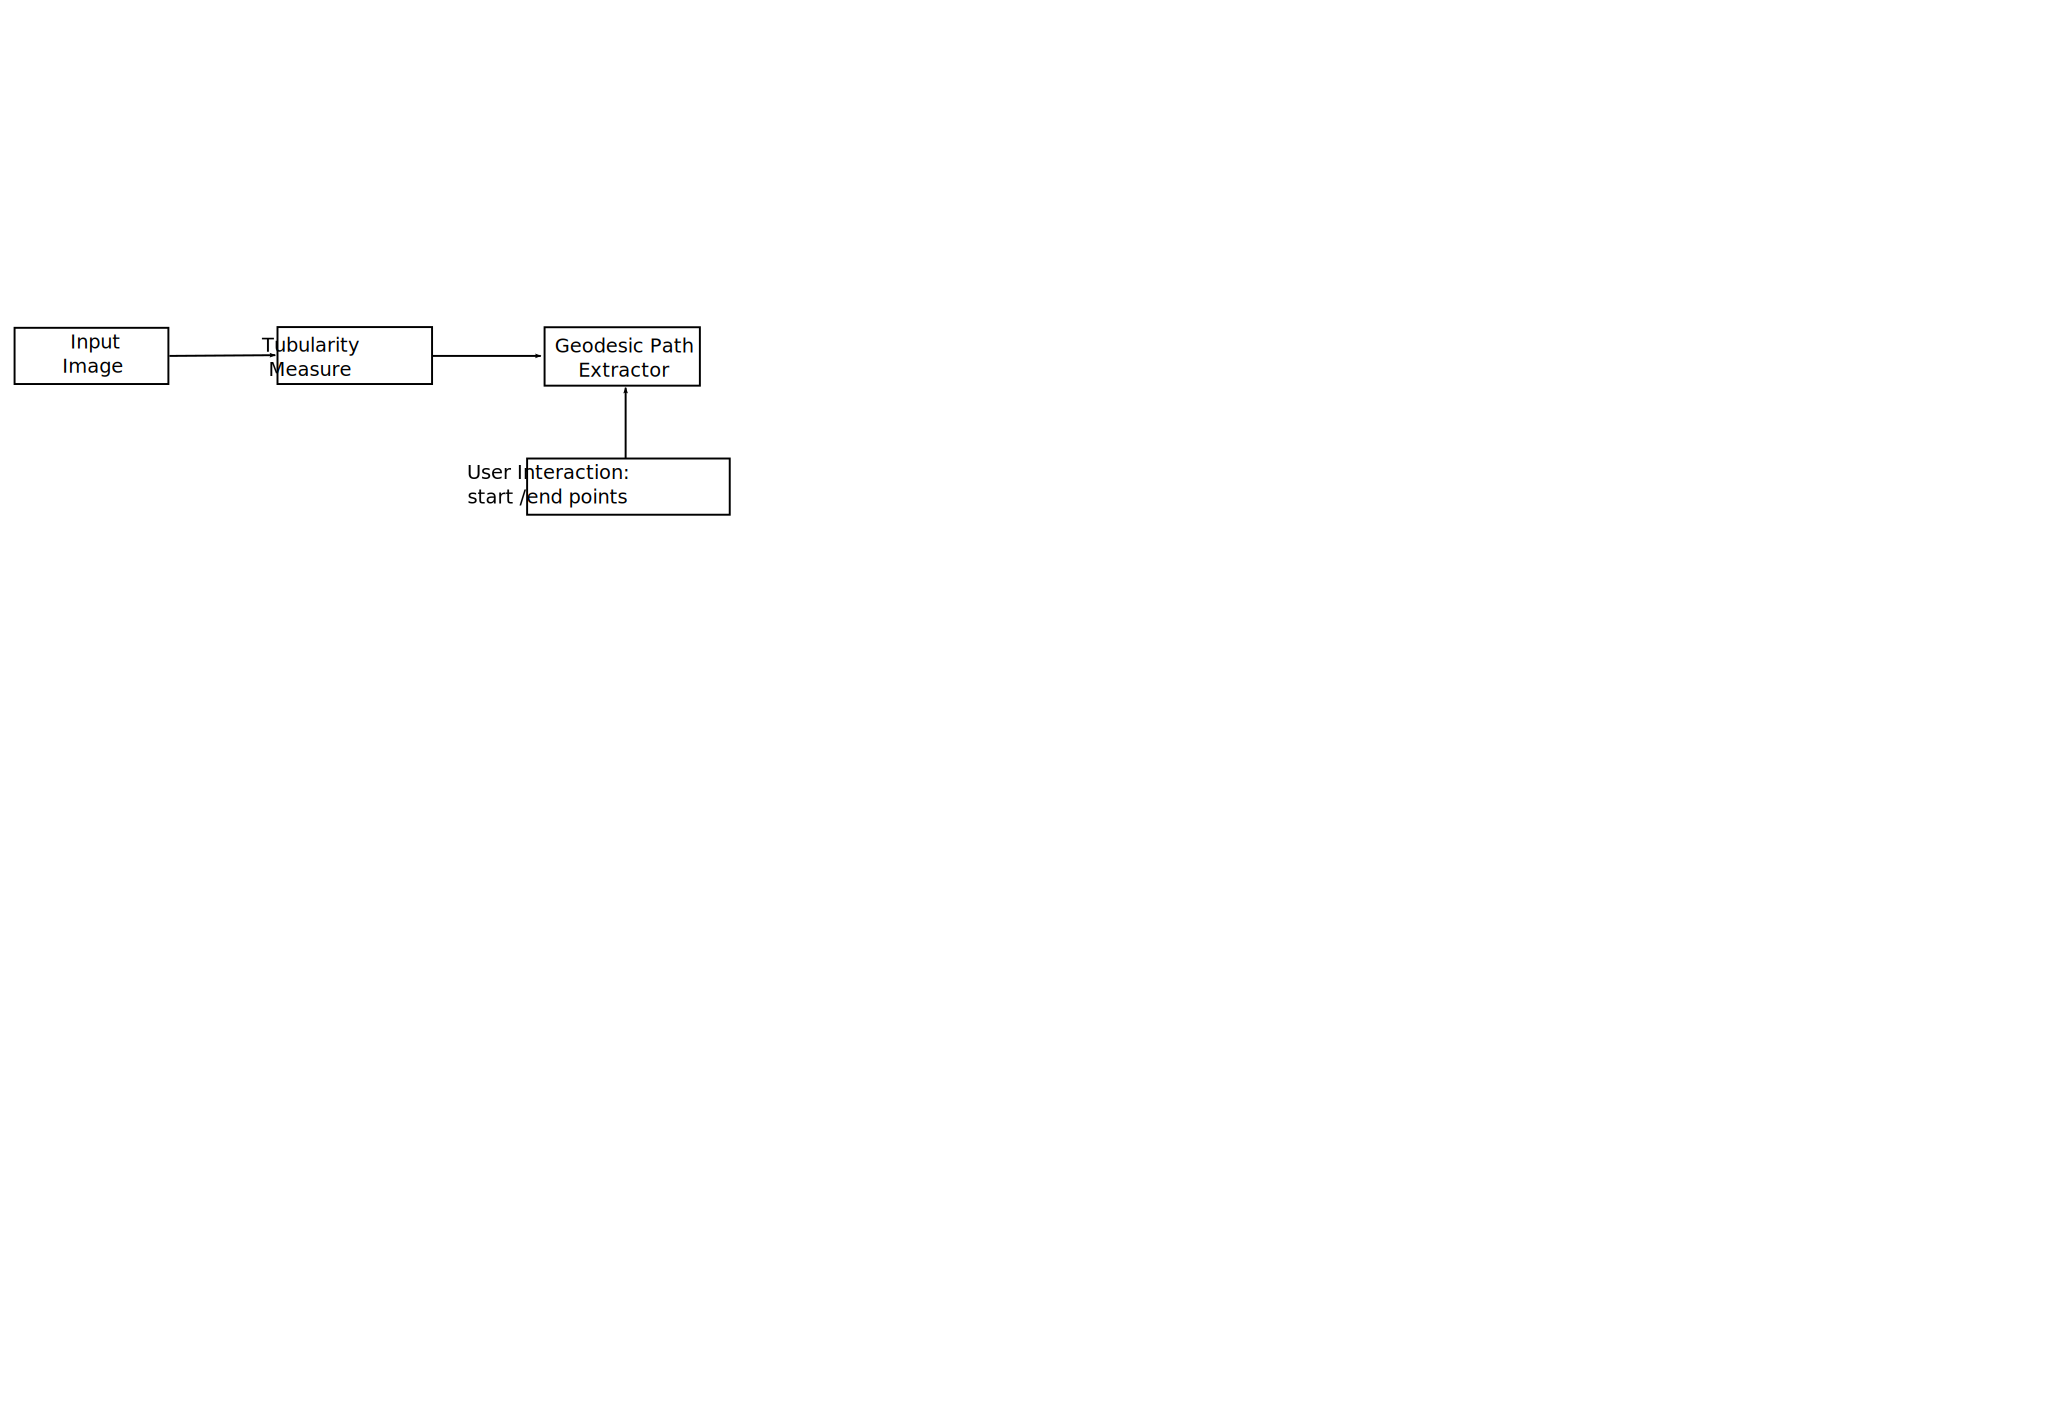
\includegraphics[width=0.5\linewidth]{Diagram}
\end{center}
%Caption
\caption{Tubular Geodesic computation pipeline.}
%Caption
\label{fig:diagram}
\end{figure}
%FFFFFFFFFFFFFFFFFFFFFFFFFFFFFFFFFFFFFFFFFFFFFFFFFFFFFFFFFFFFFFFFFFFFFFFFFFFF

Compared to the previous ITK implementation \cite{Mueller2008} for computing centrelines using the fast marching algorithm, ours has the advantage of providing at the same time the centreline and an estimate of the radius. Moreover, using our $4^{th}$ order Runge-Kutta implementation of the gradient descent step, the obtained tubular path are less prone to oscillations. Finally, in\cite{Mueller2008} the author claims that \lq\lq choosing an appropriate speed function is the most difficult part of the entire process\rq\rq. We propose an implementation that provides a well suited speed functions to extract tubular structures from 2D or 3D images.

This implementation have been incorporated in an \texttt{ImageJ/FIJI} GUI \footnote{\url{http://cvlab.epfl.ch/software/delin/index.php}} for semi-automatic tracing of tube-like structures through 3D image stacks, see figure.

%FFFFFFFFFFFFFFFFFFFFFFFFFFFFFFFFFFFFFFFFFFFFFFFFFFFFFFFFFFFFFFFFFFFFFFFFFFFF
\begin{figure}[!h]
\begin{center}		
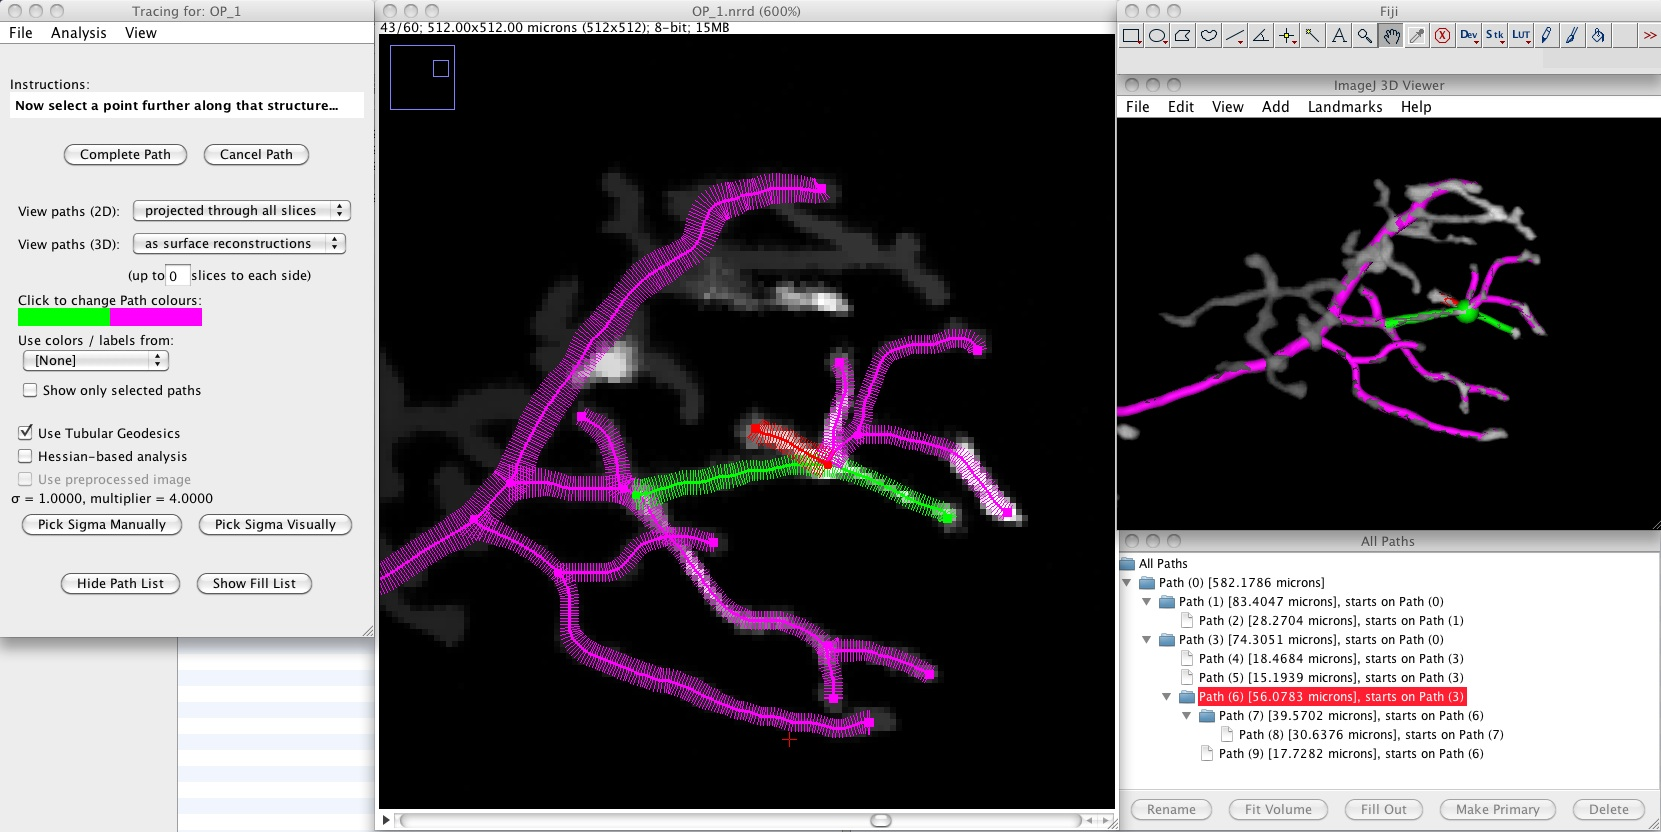
\includegraphics[width=0.70\linewidth]{DemoTubularGeo1}
\end{center}
%Caption
\vspace{-0.5cm}
\caption{Illustration of our tracing tool using the ITK implementation of the tubular geodesic extractor}
%Caption
\label{fig:diagram}
\end{figure}
%FFFFFFFFFFFFFFFFFFFFFFFFFFFFFFFFFFFFFFFFFFFFFFFFFFFFFFFFFFFFFFFFFFFFFFFFFFFF


\section{Implementation}

In \cite{Li07}, a variant of the classical, purely spatial, minimal path technique is proposed. By incorporating an extra \textit{non-spatial} dimension into the search space, a point of the 4D path (after adding the extra dimension for the 3D image) consists of three spatial coordinates plus a fourth coordinate which describes the vessel thickness at that corresponding 3D point, see figure \ref{fig:nDVesselAs} as a 2D example. Thus, each 4D point represents a sphere in 3D space, and the vessel is obtained by taking the envelope of these spheres as we move along the 3D curve. A crucial step of this method is to build an adequate tubularity measure that drives the propagation.  As opposed to \cite{Li07}, the proposed tubularity measure is a parameter free.  
%FFFFFFFFFFFFFFFFFFFFFFFFFFFFFFFFFFFFFFFFFFFFFFFFFFFFFFFFFFFFFFFFFFFFFFFFFFFF
\begin{figure}[!h]
\begin{center}		
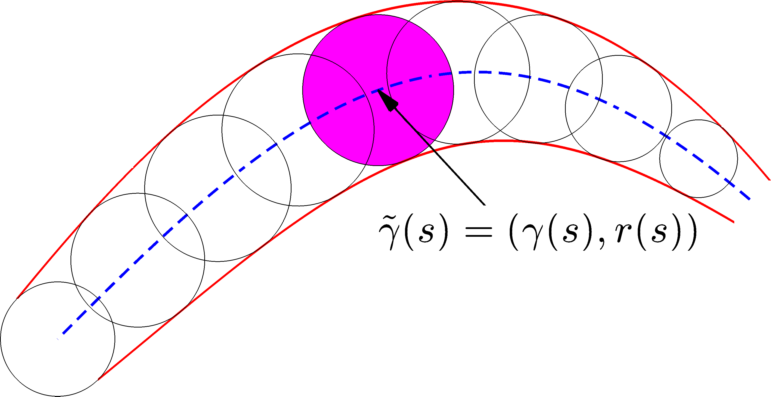
\includegraphics[width=0.5\linewidth]{SynthVessels}
\end{center}
%Caption
\caption{A tubular shape is presented as the envelope of a family of spheres or disks with continuously changing center points and radii.}
%Caption
\label{fig:nDVesselAs}
\end{figure}
%FFFFFFFFFFFFFFFFFFFFFFFFFFFFFFFFFFFFFFFFFFFFFFFFFFFFFFFFFFFFFFFFFFFFFFFFFFFF

We start by describing our implementation for computing geodesic paths. Next, we describe our implementation for computing the tubularity measure that drive the tubular geodesics. %Finally, we compare our methods reconstructions to state of the art methods. 

\subsection{Tubularity Measure}

The tubularity measure we propose to use is based on the Optimally Oriented Flux (OOF) \cite{Law08}.
At the location $\mathbf{x}$ in an image $I$, the oriented flux is the amount of the image gradient projected along the axis $\mathbf{v}$ flowing out from a 3D local sphere\footnote{Centered at point $\mathbf{x}$.} (or a 2D circle) $S_r$. It is measured as follows:
%++++++++++++++++++++++++++++++++++++++++++++++++++++++++++++++++++++++++++++
\begin{equation}
f(\mathbf{x}, \mathbf{v};r)
=\int_{\partial S_r} \left((\nabla (G*I)(\mathbf{x} + \mathbf{h})\cdot \mathbf{v})\mathbf{v}\right)
\cdot \mathbf{n} \mathrm{d}a,
\label{eqn:oflux}
\end{equation}
%++++++++++++++++++++++++++++++++++++++++++++++++++++++++++++++++++++++++++++
where $G$ is a Gaussian function with a scale factor of $1$ pixel, $r$ is the radius of the sphere (or circle), $\mathbf{h} = r \mathbf{n}$ is the relative position vector along $\partial S_r$, with $\mathbf{n}$ the outward unit normal of $\partial S_r$, and $\mathrm{d}a$ is the infinitesimal area (or length) on $\partial S_r$. Function $f$ is the flux of the smoothed image gradient $\nabla(G*I)$ projected along direction $\mathbf{v}$ toward the sphere $\partial S_r$. To detect vessels having higher intensity than the background region, one would be interested in finding the vessel direction which minimizes $f(\mathbf{x}, \mathbf{v}; r)$, i.e. we are looking for:
%++++++++++++++++++++++++++++++++++++++++++++++++++++++++++++++++++++++++++++
\begin{equation}
\arg\min\limits_{\mathbf{v}} f(\mathbf{x}, \mathbf{v};r).
\label{eqn:min}
\end{equation}
%++++++++++++++++++++++++++++++++++++++++++++++++++++++++++++++++++++++++++++
Using the divergence theorem, it can be shown that $f(\mathbf{x}, \mathbf{v};r)$ is a quadratic form on $\mathbf{v}$ and its associated matrix can be calculated using a simple convolution,
%++++++++++++++++++++++++++++++++++++++++++++++++++++++++++++++++++++++++++++
\begin{equation}\label{eqn:ofluxmatrix}
f(\mathbf{x}, \mathbf{v};r)= \mathbf{v}^{T}\,\,\left\{ I*(\partial_{i,j} G)*\mathds{1}_{S_r} (\mathbf{x})\right\}\,\, \mathbf{v} := \mathbf{v}^{T}\,\,\left\{ I*\mathbf{F}_r (\mathbf{x})\right\}\,\, \mathbf{v},
\end{equation}
%++++++++++++++++++++++++++++++++++++++++++++++++++++++++++++++++++++++++++++
where $(\partial_{i,j} G)$ is the Hessian matrix of function $G$ and $\mathds{1}_{S_r}$ is the indicator function of the sphere (or circle) $S_r$. $\mathbf{F}_r$ is called the \textit{oriented flux filter}. 

By differentiating the above equation with respect to $\mathbf{v}$, minimization of function $f$ is in turn acquired as solving a generalized eigenvalue decomposition problem. Solving the aforementioned generalized eigen decomposition problem gives $d$ eigenvalues (where $d = 2 \text{ or }3$ is the dimension of the image), $\lambda_1(\cdot)\leq \dots\leq \lambda_{d}(\cdot)$. To handle the vessels having various radii, a multi-scale approach should be used along with the OOF method. In \cite{Law08}, Law and Chung have proposed to normalize the OOF's eigenvalues by the sphere surface area when the OOF method is incorporated in a multi-scale approach for 3D image volumes. In the 2D case the eigenvalues are normalized by the circle perimeter $2\pi r$. In the 3D case the eigenvalues are normalized by the sphere area $4\pi r^2$.

We propose an ITK implementation of the oriented flux filter using the analytical expression of the OOF~\cite{Law08}. First, the filter \code{itk::OrientedFluxMatrixImageFilter} implements the normalized convolution $I*\mathbf{F}_r/r^{d-1}$, $d$ being the dimension of the image. This filter is templated over the input image type and the output image type for which the default pixel type is \code{itk::SymmetricSecondRankTensor}, since the output is a symmetric matrix. Then, the filter \code{itk::MultiScaleOrientedFluxBasedMeasureImageFilter} implements multi-scale oriented flux measures by combining the eigenvalues of the oriented flux matrix. This filter is very similar to \code{itk::MultiScaleHessianBasedMeasureImageFilter}. We added a few options like the possibility of generating the scale estimate at each voxel location and a scale space tubularity measure that could be used for tracing geodesic tubes.
The proposed tubularity measures, \code{itk::OrientedFluxCrossSectionTraceMeasure}, sums the $(d-1)$ eigenvalues that correspond to the cross-section of the tubular structure. For a complete example, one can see the provided code: \code{itkMultiScaleOrientedFluxBasedMeasureImageFilter.cxx}.

\subsection{Tubular Geodesic}
A \textit{tubular geodesic} is a path, linking two points, that globally minimizes an energy functional weighted by a tubularity measure. Without loss of generality and in order to simplify notations we will assume hereinafter that a path $\gamma$ is parametrized along its length (i.e $\|\gamma'\| = 1$). The energy minimized by a geodesic is under the form:
%++++++++++++++++++++++++++++++++++++++++++++++++++++++++++++++++++++++++++++
\begin{equation}\label{eqn:IsotropicEnergy}
E(\gamma)=\int_{\gamma} \mathcal{P}\big( \gamma(s) \big)\mathrm{d}s.
\end{equation}
%++++++++++++++++++++++++++++++++++++++++++++++++++++++++++++++++++++++++++++
where $\mathcal{P} > 0$ is a tubularity measure that will be described later.



A geodesic path connecting two 4D tubular points $\mathbf{p}_{1}$ and $\mathbf{p}_{2}$, globally minimizes the above energy (\ref{eqn:IsotropicEnergy}) and is noted $\mathcal{C}_{\mathbf{p}_{1},\mathbf{p}_{2}}$.

The solution of this minimization problem is obtained through the computation of the \textit{geodesic distance} $\mathcal{U}:\Omega\rightarrow\mathbb{R}^{+}$ associated to~$\mathbf{p}_{1}$ on the domain $\Omega\subset\mathbb{R}^d$ ( $d =  4$ for extracting tubes in 3D images). The geodesic distance is the minimal energy integrated along a path between $\mathbf{p}_{1}$ and any point $\mathbf{x}$ of the domain $\Omega$ :
%++++++++++++++++++++++++++++++++++++++++++++++++++++++++++++++++++++++++++++
\begin{equation}\label{eqn:minimalactionmap1}
\forall~\mathbf{x}\in\Omega,~\mathcal{U}(\mathbf{x})=
\min_{\gamma \in \mathcal{A}_{\mathbf{p}_{1},\mathbf{x}}}
\Bigg\{ \int_{\gamma} \mathcal{P}\big(\gamma(s) \big) \mathrm{d}s \Bigg\}~,
\end{equation}
%++++++++++++++++++++++++++++++++++++++++++++++++++++++++++++++++++++++++++++
where $\mathcal{A}_{\mathbf{p}_{1},\mathbf{x}}$ is the set of paths linking $\mathbf{x}$ to $\mathbf{p}_{1}$.
The values of $\mathcal{U}$ may be regarded as the arrival times of a front propagating 
from the source $\mathbf{p}_{1}$ with velocity  $1/\mathcal{P}$.
$\mathcal{U}$ satisfies the Eikonal equation
%++++++++++++++++++++++++++++++++++++++++++++++++++++++++++++++++++++++++++++
\begin{equation}\label{eqn:eikonal1}
\|\nabla \mathcal{U}(\mathbf{x})\| =  \mathcal{P}\text{ for }~\mathbf{x}\in\Omega,\text{ and }   \mathcal{U}(\mathbf{p}_{1}) = 0,
\end{equation}
%++++++++++++++++++++++++++++++++++++++++++++++++++++++++++++++++++++++++++++
The map $\mathcal{U}$ has only one local minimum, the source point $\mathbf{p}_{1}$, and its flow lines satisfy the Euler-Lagrange equation of functional (\ref{eqn:IsotropicEnergy}). Thus, the minimal path $\mathcal{C}_{\mathbf{p}_{1},\mathbf{p}_{2}}$ can be retrieved with a simple gradient descent on $\mathcal{U}$ from $\mathbf{p}_{2}$ to $\mathbf{p}_{1}$, solving the following ordinary differential equation with standard numerical methods like Heun's or Runge-Kutta's :
%++++++++++++++++++++++++++++++++++++++++++++++++++++++++++++++++++++++++++++
\begin{equation}\label{eqn:gradientdescent1}
\displaystyle\frac{\mathrm{d} \mathcal{C}_{\mathbf{p}_{1},\mathbf{p}_{2}}}{\mathrm{d}s} (s) \propto 
 -\nabla\mathcal{U}\big(\mathcal{C}_{\mathbf{p}_{1},\mathbf{p}_{2}}(s)\big),\text{ with }\mathcal{C}_{\mathbf{p}_{1},\mathbf{p}_{2}}(0) = \mathbf{p}_{2}.
\end{equation}
%++++++++++++++++++++++++++++++++++++++++++++++++++++++++++++++++++++++++++++

The main filter to compute a geodesic path given a tubularity measure is \code{itk::TubularMetricToPathFilter}, which is a subclass of \code{itk::ImageToPathFilter}. \code{itk::TubularMetricToPathFilter} expects one start point, a set of end points, and a tubularity measure that drive the propagation (an image with real non-negative values). A front is launched from the start point using the fast marching filter and the propagation is stopped as soon as the endpoints are reached. To achieve this step, we used the \code{itk::FastMarchingUpwindGradientImageFilter}, so that the estimated gradient directions are used to back propagate from the endpoints to the start point in order to obtain the tubular path. The back propagation could be done using a discrete neighborhood iterator, \code{itk::IterateNeighborhoodCharacteristicDirectionsToPathFilter}, or a fixed step gradient descent optimizer, \code{itk::FixedStepDescentCharacteristicDirectionsToPathFilter}, similar to the ones proposed in \cite{Mueller2008}. In addition to those tow filters, we implemented the $4^{th}$ order Runge�Kutta back propagation method so that the oscillations are much more reduced. 

 (which are parallel to the  of the geodesic distances for the current isotropic case)


%
%For the implementation, first describe quickly \code{PolyLineParametricTubularPath}.
%Second, recall that equation (\ref{eqn:eikonal1}) is solved using the fast marching algorithm
%\listcpluspluspsnip
%\lstinputlisting[float,label=typedef:FM,linerange={89-92}]
%                 {../src/itkTubularMetricToPathFilter.h}
%                 
%\listcpluspluspsnip                 
%\lstinputlisting[float,label=lst:Slice1,linerange={229-231,240-249,251-267}]
%                 {../src/itkTubularMetricToPathFilter.hxx}
%
%The implementation of the geodesic path extractor consists of one filter 
%\listcpluspluspsnip
%\lstinputlisting[float,label=lst:Slice1,linerange={259-261}]
%                 {../src/itkTubularMetricToPathFilter.cxx}
%
%In this project, we implemented a number of auxiliary functions and filters, nevertheless only two filters are expected to be used:
%\begin{itemize}
%\item[$\bullet$] \code{itk::MultiScaleOrientedFluxBasedMeasureFFTImageFilter}
%\item[$\bullet$] \code{itk::TubularMetricToPathFilter}
%\end{itemize}



\section{Examples}

\section{Conclusion}
In this paper, we described an implementation of geodesic tubes for ITK. The framework allows a user to construct a scale space metric well suited for tubular structure. This metric is used to extract shortest tubes between points provided by a user, that is a centerline and width estimates. For suggestion or bugs, feel free to contact the authors.  

\bibliographystyle{plain}
\bibliography{TubularGeodesicITK}


\end{document}
